% Общая конфигурация
%%%%%%%%%%%%%%%%%%%%%%%%%%%%%%%%%%%%%%%%%%%%%%%%%%%%%%%%%%%%%%%%%%%%%
%% ���������������� ����
%%%%%%%%%%%%%%%%%%%%%%%%%%%%%%%%%%%%%%%%%%%%%%%%%%%%%%%%%%%%%%%%%%%%%
%%
%%

%%%%%%%%%%%%%%%%%%%%%%%%%%%%%%%%%%%%%%%%%%%%%%%%%%%%%%%%%%%%%%%%%%%%%
%% ���������� � ����������� �������� ����� KOMA-Sript
\documentclass{scrreprt}
\KOMAoptions{
  fontsize = 12pt, 
  numbers = periodatend, 
  chapteratlists,
  headings = chapterprefix,
  toc = bib,
  captions = tableheading,
  draft
}

%% ����������� ������ �������� � �������� � ��������
\setkomafont{captionlabel}{\bfseries\sffamily}
\setkomafont{caption}{\sffamily}
\renewcommand*{\captionformat}{~}

%% ����������� ������ ������
\deffootnote[1.5em]{0em}{1em}{\textsuperscript{\thefootnotemark}\,}

%% ��������� �������������� �� ������������� ����������� ������� \float@addtolist,
%% ������� ������������, ��������, � ������ listings
\usepackage{scrhack}

%%%%%%%%%%%%%%%%%%%%%%%%%%%%%%%%%%%%%%%%%%%%%%%%%%%%%%%%%%%%%%%%%%%%%
%% ����������� ���������� � ����
\defaulthyphenchar=127
\usepackage{cmap}
\usepackage[T2A]{fontenc}
\usepackage[cp1251]{inputenc}
\usepackage[english, greek, russian]{babel}

%% ����������� ���� � ������� ��� ��������
\usepackage{geometry}   
\geometry{
  left = 3cm,
  right = 2cm,
  top = 2cm,
  bottom = 2cm,
  headheight = 1cm,
  headsep = 0.5cm,
  footskip = 1cm
}

%% ������������� ���������� ����������� ��������
\usepackage{setspace}
\onehalfspacing

%% �������� ������ � ������� ������
\usepackage{indentfirst}
%5 ������������� �������� ���������� �������
\setlength{\parindent}{1cm} 

%% ���������������� (���������� ������������ ������)
\usepackage[protrusion, expansion]{microtype}

%% ���������� � ����������� ����� ��� �����������
\usepackage[hang, raggedright, small]{subfigure}
% ���������� ������������ �������� �������
\renewcommand{\thesubfigure}{\emph{\asbuk{subfigure}}}
\makeatletter
  \renewcommand{\p@subfigure}{\thefigure}
  \renewcommand{\@thesubfigure}{\emph{\asbuk{subfigure}})~}
\makeatother

\renewcommand{\thesubtable}{\emph{\asbuk{subtable}}}
\makeatletter
  \renewcommand{\p@subtable}{\thetable}
  \renewcommand{\@thesubtable}{\emph{\asbuk{subtable}})~}
\makeatother

%% �����, ������� �� ��������� ��������� ������� �������� �� ������� ��������
\usepackage[section]{placeins}
\makeatletter 
% ��������, ����� ��� �� �������� � �� ������� �����������
\AtBeginDocument{%
  \expandafter\renewcommand\expandafter\subsection\expandafter
    {\expandafter\@fb@subsecFB\subsection}%
  \newcommand\@fb@subsecFB{\FloatBarrier
  \gdef\@fb@afterHHook{\@fb@topbarrier \gdef\@fb@afterHHook{}}}
  \g@addto@macro\@afterheading{\@fb@afterHHook}
  \gdef\@fb@afterHHook{}
}
\makeatother 

%% ���������� ����� TikZ � �������������� ������ � ���� 
\usepackage{tikz}
\makeatletter
\pgfdeclareshape{fflop} {
  \inheritsavedanchors[from=rectangle]
  \inheritanchorborder[from=rectangle]
  \inheritanchor[from=rectangle] {center}
  \inheritanchor[from=rectangle] {north}
  \inheritanchor[from=rectangle] {south}
  \inheritanchor[from=rectangle] {west}
  \inheritanchor[from=rectangle] {east}

  \backgroundpath{
    % Store lower right in xa/ya and upper right in xb/yb
    \southwest \pgf@xa=\pgf@x \pgf@ya=\pgf@y
    \northeast \pgf@xb=\pgf@x \pgf@yb=\pgf@y

    \pgf@xc=.5\wd\pgfnodeparttextbox
    \pgf@yc=\pgf@ya \advance\pgf@yc by 10pt
    % Rectangle
    \pgfpathmoveto{\pgfpoint{\pgf@xa}{\pgf@ya}}
    \pgfpathlineto{\pgfpoint{\pgf@xa}{\pgf@yb}}
    \pgfpathlineto{\pgfpoint{\pgf@xb}{\pgf@yb}}
    \pgfpathlineto{\pgfpoint{\pgf@xb}{\pgf@yb}}
    \pgfpathlineto{\pgfpoint{\pgf@xb}{\pgf@ya}}
    \pgfpathclose
    % Add triangle at the bottom
    \pgfpathmoveto{\pgfpoint{\pgf@xa}{\pgf@ya}}
    \pgfpathlineto{\pgfpoint{\pgf@xc}{\pgf@yc}}
    \pgfpathlineto{\pgfpoint{\pgf@xb}{\pgf@ya}}
  }
}
\makeatother

\usetikzlibrary{
  shapes,
  arrows,
  intersections,
  positioning,
  fit
}
\tikzset{
  font = \small\sffamily,
  inner sep = 5pt,
  node distance = 20pt,
  trapezium stretches body,
  every fit/.append style = text badly centered,
  pre/.style = {<-, shorten <=1pt, >=stealth'},
  post/.style = {->, shorten >=1pt, >=stealth'},
  block/.style = {
    draw = #1!80,
    fill = #1!20,
    align = center,
    text badly centered
  },
  block/.default = blue,
  flop/.style = {
    block = gray,
    shape = fflop,
    minimum width = .5cm,
    minimum height = 1.5cm
  },
  port/.style = {
    block = red,
    font = \rmfamily,
    text width = .3cm,
    minimum height = .5cm
  },
  mux/.style = {
    block = gray,
    trapezium,
    shape border uses incircle,
    shape border rotate = -90,
    minimum width = 1cm
  },
  demux/.style = {
    mux,
    shape border rotate = 90
  },
  FSM/.style = {
    block = red,
    rounded corners,
    minimum height = 1cm,
    minimum width = 1.5cm
  },
  label/.style = {
    font = \scriptsize\sffamily,
    inner sep = 1pt
  },
  exchange/.style = {
    <->,
    shorten <=1pt,
    shorten >=1pt,
    >=fast cap,
    line width = 5pt
  }, 
  arith/.style = {
    block,
    minimum width =  1.5cm,
    minimum height = 1.5cm
  },
  module/.style = {
    draw = black!50,
    fill = yellow!20,
    rounded corners,
    inner sep = 10pt,
    dashed
  }
}
% ����������� ����
\pgfdeclarelayer{background}
\pgfdeclarelayer{foreground}
\pgfsetlayers{background,main,foreground}

%% ���������� � ����������� ����� ��� ����������������� �������
\usepackage{enumitem}
% ������������ ����� ������� ��� ������� � �������� �������
\makeatletter
  \AddEnumerateCounter{\asbuk}{\@asbuk}{\cyrzh}
  \AddEnumerateCounter{\Asbuk}{\@Asbuk}{\CYRZH}
\makeatother
% ������ ���������� �� � ����� ������ � ����������� ������������
\setlist{leftmargin = *, nolistsep}
% ��� ������� ������� ������ ������������� �����, ������ ���������
\setlist[1]{labelindent = \parindent}
% ������������� �� ���������� ������ ���� ���� 1)
\setenumerate{label = \arabic*)}
% �������� ��� ������� �� ��������� ������ ����
\setitemize{label = \textemdash}

%% ����������� ������ ��� ������ � ���������
\usepackage{longtable, array, colortbl}
\usepackage{booktabs}
\usepackage{multirow}
\newcolumntype{L}{>{$}l<{$}}
\newcolumntype{C}{>{$}c<{$}}

% �������������� (math) �������
\newcolumntype{m}[1]{>{\raggedright\arraybackslash $}p{#1}<{$}}
% ��������� (text) �������
\newcolumntype{t}[1]{>{\raggedright\arraybackslash}p{#1}<{}}
\renewcommand{\arraystretch}{1.3}
\renewcommand{\arrayrulewidth}{0.6pt}
% ������������� ���� ��� ����� ����� �������
\colorlet{tableheadcolor}{gray!25}

\usepackage{lscape, pdflscape} 
\usepackage{amsmath, amssymb, ifthen, calc}

\usepackage[group-minimum-digits = 4]{siunitx}

%% ���������� ����� xspace
\usepackage{xspace}
% ����� �� ������ ������ ����� ��������� � ����� �������
\xspaceaddexceptions{<< >> ,, ``}

%% ���������� ����� ���
\usepackage{datetime}
% ������������� ������ ����
\ddmmyydate

%% ���������� ����� ��� ����������� ��������� ��������
\usepackage{listings}

\renewcommand{\lstlistingname}{�������}
% ������ ����� ����� ������ ����� ���������
\makeatletter
  \AtBeginDocument{\renewcommand \thelstlisting{\thechapter.\@arabic\c@lstlisting\autodot}}
\makeatother
% ����������� ����� ��-���������


\DeclareNewTOC[
  type = codebox,
  types = codeboxes,
  float,
  floatpos = h,
  floattype = 4,
  nonfloat,
  name = �������,
  listname = {������ ���������}
]{lor}
\setuptoc{lor}{chapteratlist}
\makeatletter
  \AtBeginDocument{\renewcommand \thecodebox{\thechapter.\@arabic\c@codebox}}
\makeatother

%% ���������� ����� ��� �������������� ����������
\usepackage[noend]{algorithmic}
\algsetup{
  linenosize = \tiny,
  linenodelimiter = \ 
}
% ������������ �������� �����
\def\algorithmicrequire{\textbf{����:}}
\def\algorithmicensure{\textbf{�����:}}
\def\algorithmicif{\textbf{����}}
\def\algorithmicthen{\textbf{��}}
\def\algorithmicelse{\textbf{�����}}
\def\algorithmicelsif{\textbf{����� ����}}
\def\algorithmicfor{\textbf{���}}
\def\algorithmicforall{\textbf{��� ����}}
\def\algorithmicdo{}
\def\algorithmicwhile{\textbf{����}}
\def\algorithmicrepeat{\textbf{���������}}
\def\algorithmicuntil{\textbf{����}}
\def\algorithmicloop{\textbf{����}}
\def\algorithmiccomment#1{\quad/\!/ \textit{#1}}

%% ����������� ����� ��� ����������� �����������
\usepackage{hyperref}
\urlstyle{sf}

% ������ ���������� ������� �������� �����
\makeatletter
\g@addto@macro{\Url@acthash}{\Url@Edit\Url@String{//}{/\kern-0.2em/}}
\makeatother

% ������� �������������� ���������� �����
\usepackage{mathrsfs}

% ���������� �����
\usepackage{yfonts}

% ���������
\usepackage{pb-diagram}

% ��� ������������� ������������
\usepackage{verbatim}

%% ������ ������� �������� (�������, ��������, ������, ���. �������) � ���������
\usepackage{totcount, etoolbox}
\regtotcounter{page}
\regtotcounter{figure}
\regtotcounter{table}
\regtotcounter{codebox}
\regtotcounter{enumiv}

\newcounter{totfigures}
\newcounter{tottables}
\newcounter{totlistings}

\providecommand\totfig{} 
\providecommand\tottab{}
\providecommand\totlst{}

\makeatletter
\AtEndDocument{%
  \addtocounter{totfigures}{\value{figure}}%
  \addtocounter{tottables}{\value{table}}%
  \addtocounter{totlistings}{\value{codebox}}%
  \immediate\write\@mainaux{%
    \string\gdef\string\totfig{\number\value{totfigures}}%
    \string\gdef\string\tottab{\number\value{tottables}}%
    \string\gdef\string\totlst{\number\value{totlistings}}%
  }%
}
\makeatother

\pretocmd{\chapter}{\addtocounter{totfigures}{\value{figure}}\setcounter{figure}{0}}{}{}
\pretocmd{\chapter}{\addtocounter{tottables}{\value{table}}\setcounter{table}{0}}{}{} 
\pretocmd{\chapter}{\addtocounter{totlistings}{\value{codebox}}\setcounter{codebox}{0}}{}{}

% ����� ��� �������� ���������� ����������
\usepackage{makeidx}

% ����� ��� ���������
\usepackage{epigraph}

% ����� ��� ������ �� ��������� ��������
\usepackage{lastpage}

% ������� � ������ ��� ������
\usepackage{textcomp}

% Subsection ��� ���������
\makeatletter
\newcommand*\addsubsec{\secdef\@addsubsec\@saddsubsec}
\newcommand*{\@addsubsec}{}
\def\@addsubsec[#1]#2{\subsection*{#2}\addcontentsline{toc}{subsection}{#1}
  \if@twoside\ifx\@mkboth\markboth\markright{#1}\fi\fi
}
\newcommand*{\@saddsubsec}[1]{\subsection*{#1}\@mkboth{}{}}
\makeatother

% Subsubsection ��� ���������
\makeatletter
\newcommand*\addsubsubsec{\secdef\@addsubsubsec\@saddsubsubsec}
\newcommand*{\@addsubsubsec}{}
\def\@addsubsubsec[#1]#2{\subsubsection*{#2}\addcontentsline{toc}{subsubsection}{#1}
  \if@twoside\ifx\@mkboth\markboth\markright{#1}\fi\fi
}
\newcommand*{\@saddsubsubsec}[1]{\subsubsection*{#1}\@mkboth{}{}}
\makeatother

%%%%%%%%%%%%%%%%%%%%%%%%%%%%%%%%%%%%%%%%%%%%%%%%%%%%%%%%%%%%%%%%%%%%%
%% ������ ���������� �������� � �������������� ��������, �����
%% ���� �������� ����������� �� ����� ������ 
%%
%% ��� ������� �� ���� ������ 'russmath', �����: leontiev@aport.ru
%%
\newif\ifBrkFlag
\def\allowmathbreak{\global\BrkFlagtrue\global\relpenalty=10000\global\binoppenalty=10000}
\def\cancelmathbreak{\global\BrkFlagfalse\global\relpenalty=500\global\binoppenalty=700}
\allowmathbreak

\makeatletter
\def\m@th{\mathsurround=0pt}
\def\@thick{\hbox{\m@th$\mskip\thickmuskip$}}
\def\@med{\hbox{\m@th$\mskip\medmuskip$}}

\def\brel#1{\ifBrkFlag\discretionary{\@thick\hbox{\m@th$#1$}}{}{}\fi #1}
\def\bbin#1{\ifBrkFlag\discretionary{\@med\hbox{\m@th$#1$}}{}{}\fi #1}
\makeatother
%%%%%%%%%%%%%%%%%%%%%%%%%%%%%%%%%%%%%%%%%%%%%%%%%%%%%%%%%%%%%%%%%%%%%
%% �������
%%%%%%%%%%%%%%%%%%%%%%%%%%%%%%%%%%%%%%%%%%%%%%%%%%%%%%%%%%%%%%%%%%%%%
%%
%%

%% ��������� ����������
% Exapmli gratia (eg.) = �������� (����.)
\newcommand{\eg}{��������,\xspace}
\newcommand{\Eg}{��������,\xspace}
% Et cetera (etc.) = � ��� ����� (� �.�.)
\renewcommand{\etc}{�~�.\,�.\xspace}
% Id est (i.e.) = �� ���� (�.�.)
\newcommand{\ie}{�.\,�.\xspace}
\newcommand{\Ie}{�.\,�.\xspace}
% Et alii (et al.) = � ������ (� ��.)
\newcommand{\etal}{�~��.\xspace}

%% ������� ��� ��������
\newcommand{\fixme}{FIXME}
\newcommand{\unref}{[???]}

\newcommand{\kips}{$\text{��}/\text{�}$\xspace}

%% �������
%% ��� ��������� ������
\newcommand{\strong}[1]{\textbf{#1}}
% ��� ������� ����������� ���� � ��������������
\newcommand{\foreigne}[1]{\mbox{����.}~\emph{\foreignlanguage{english}{#1}}} % ����������
\newcommand{\foreigng}[1]{\mbox{����.}~\foreignlanguage{greek}{#1}} % ���������
\newcommand{\foreignl}[1]{\mbox{���.}~\emph{\foreignlanguage{latin}{#1}}} % ���������
\newcommand{\foreignfrak}[1]{\mbox{���.}~\textfrak{#1}} % �������� ����������
%% ��� ��������� �������� ���� (��������)
\newcommand{\keyword}[2][russian]{\textsf{\foreignlanguage{#1}{#2}}}
\newcommand{\keyworde}[2]{\textsf{#1} (\foreigne{#2})}
\newcommand{\keywordg}[2]{\textsf{#1} (\foreigng{#2})}
\newcommand{\keywordl}[2]{\textsf{#1} (\foreignl{#2})}
\newcommand{\keywordfrak}[2]{\textsf{#1} (\foreignfrak{#2})}

%% ��� ������� ����������
\newcommand{\gap}{\ensuremath{\langle\ldots\rangle}\xspace}
%% ��� ������� ������ �� ������� � �������
\newcommand{\seefig}[1]{��.~���.~\ref{#1}}
\newcommand{\fig}[1]{���.~\ref{#1}}
\newcommand{\seetab}[1]{��.~����.~\ref{#1}}
\newcommand{\tab}[1]{����.~\ref{#1}}

%% ��������� ��� ������� ������� ����� �� ��������� ������
\newenvironment{mquote}[1][russian]{%
  \bigskip%
  \begin{addmargin}{1.1\parindent}%
  \setlength{\parindent}{0pt}%
  \setlength{\parskip}{\smallskipamount}%
  \selectlanguage{#1}%
  \sffamily\small%
}{
  \end{addmargin}%
  \bigskip%
}

%% ����� �������� ������� ��������� �������� ����� C++
\newcommand{\CPP}{C\kern-.05em\raise.23ex\hbox{+\kern-.05em+}\xspace}
\newcommand{\CCPP}{C/C\kern-.05em\raise.23ex\hbox{+\kern-.05em+}\xspace}

\newcommand{\midtilde}{\raise-0.5ex\hbox{\textasciitilde}}

%%%%%%%%%%%%%%%%%%%%%%%%%%%%%%%%%%%%%%%%%%%%%%%%%%%%%%%%%%%%%%%%%%%%%
%% ������ ���������� �������� � �������������� ��������, �����
%% ���� �������� ����������� �� ����� ������ 
%%
%% ��� ������� �� ���� ������ 'russmath', �����: leontiev@aport.ru
%%
\newif\ifBrkFlag
\def\allowmathbreak{\global\BrkFlagtrue\global\relpenalty=10000\global\binoppenalty=10000}
\def\cancelmathbreak{\global\BrkFlagfalse\global\relpenalty=500\global\binoppenalty=700}
\allowmathbreak

\makeatletter
\def\m@th{\mathsurround=0pt}
\def\@thick{\hbox{\m@th$\mskip\thickmuskip$}}
\def\@med{\hbox{\m@th$\mskip\medmuskip$}}

\def\brel#1{\ifBrkFlag\discretionary{\@thick\hbox{\m@th$#1$}}{}{}\fi #1}
\def\bbin#1{\ifBrkFlag\discretionary{\@med\hbox{\m@th$#1$}}{}{}\fi #1}
\makeatother

\renewcommand{\land}{\bbin{\mathbin{\&}}}
\renewcommand{\lor}{\bbin{\mathbin{\vee}}}
%% ����������
\newcommand{\impl}{\bbin{\mathbin{\Rightarrow}}}
%% ��������������
\newcommand{\equi}{\bbin{\mathbin{\Leftrightarrow}}}
%% �������� ���������� (converse implication)
\newcommand{\coimpl}{\bbin{\mathbin{\Leftarrow}}}

\newcommand{\bin}{\brel{\in}}
\newcommand{\nin}{\brel{\notin}}
%% ������ ������� ��������� (empty set)
\newcommand{\es}{\varnothing}
%% ��������� 
\newcommand{\eq}{\brel{=}}
%% ����������� 
\renewcommand{\neq}{\brel{\ne}}
%% ������ ��� ����� (greater or equal)
\renewcommand{\ge}{\brel{>}}
\renewcommand{\geq}{\brel{\geqslant}}
%% ������ ��� ����� (less or equal)
\renewcommand{\le}{\brel{<}}
\renewcommand{\leq}{\brel{\leqslant}}
%% ������� ������������
\newcommand{\subs}{\brel{\subset}}
%% ������������
\newcommand{\subseq}{\brel{\subseteq}}
%% �������� (without)
\newcommand{\wo}{\bbin{\setminus}}
%% �������������� ��������
\newcommand{\swo}{\bbin{\mathbin{\div}}}
%% ��������� ������������
\newcommand{\dec}{\bbin{\times}}
%% ����������� ������� �������� ����� ���������� � �������
\makeatletter
\newcommand{\listnopagebreak}{\par\nobreak\@afterheading}
\makeatother
%% �� � ����� ����� ���
\newcommand{\bc}{��\,�.\,�.}
\newcommand{\ad}{�.\,�.}

%% (���. 99)
\newcommand{\pagerefrus}[1]{(���.\,\pageref{#1})}
%% ����� natbib ������������ ��� ��������������� ������� \bibsection,
%% ����� ��������� ������ ����������, �������� ������� multibib, 
%% ���������� �� ����� ������ (\chapter), � ����� �������� (\section)
%% ����� ���� ����� ��������� ���������� ������ cite (sort&compress)
\usepackage[numbers, square, comma, sort&compress]{natbib}
% ������ ������ ��������� ������ ���������� � [1] �� 1.
\makeatletter\renewcommand\@biblabel[1]{#1.}\makeatother
% ������ ����� �� ������
\renewcommand\bibsection{\addsec*{\refname}}

%% ���������� ����� multibib, ����� ������� ������ ���������� �� �����
\usepackage{multibib}
% ���������� �������� � ���� ��� �������� ������ ����������
\newcites{book}{����������}
\newcites{article}{������}
\newcites{diss}{����������� � ������������}
\newcites{online}{������-���������}
\newcites{patent}{�������}

%% ������������� ����� ������ ���������� ���� 7.0.5-2008
\providecommand*{\BibEmph}[1]{\emph{#1}}


% Названия
\newcommand{\worktitle}{Пути и способы реализации компьютерной IP-телефонии в сетях ЭВМ}
\newcommand{\worksubject}{Реферат по курсу <<Архитектура и технологии сетей>>}

% Настраиваем параметры документа
\hypersetup{
  unicode,
  colorlinks,
  linkcolor = blue,
  citecolor = red,
  bookmarksopen = true,
  bookmarksnumbered = true,
  bookmarksopenlevel = 1,
  pdftitle = {\worktitle},
  pdfauthor = {Павел Крюков <kryukov@frtk.ru>},
  pdfsubject = {\worksubject},
  pdfkeywords = {гидродинамика, жидкость, несжимаемая, теплопроводность},
  pdfcreator = {LaTeX 2e with TeXnicCenter 2.0},
  pdflang = {ru-RU},
  pdfpagelayout = {SinglePage}
}

\begin{document}

%% Титульный лист
%%%%%%%%%%%%%%%%%%%%%%%%%%%%%%%%%%%%%%%%%%%%%%%%%%%%%%%%%%%%%%%%%%%%%
%% ��������� ����
%%%%%%%%%%%%%%%%%%%%%%%%%%%%%%%%%%%%%%%%%%%%%%%%%%%%%%%%%%%%%%%%%%%%%

%% �������� ������ ������ ���� ��������
\newgeometry{left=3cm, right=2cm, top=2cm, bottom=1cm} 
\onehalfspacing

\begin{titlepage}

\begin{center}
  ������������ ����������� �~����� ���������� ���������\\
  ���������� ������"=����������� �������� (��������������� �����������)\\
  ��������� ������������ �~�����������\\
  \textsf{������� <<����������������� ����������>>}

  \begin{flushright}
    \textsf{��� 004.77}
    %\textit{��~������ ��������}
  \end{flushright}

  \vspace{15mm}

  \bigskip
  \textsf{\worksubject\ ��~����:}\\
  \bigskip
  {\LARGE\sffamily\bfseries
    \worktitle
  }

\end{center}

\vspace*{\fill}
\begin{flushright}
  \newlength{\signline}
  \newlength{\signskip}
  \newcommand{\signtext}{{\footnotesize\sffamily(������� �~����)}}
  \setlength{\signline}{50mm}
  \setlength{\signskip}{\signline-\widthof{\signtext}}
  \newcommand{\signplace}{\bigskip\rule{\signline}{.6pt}\\[-2mm]\signtext\hspace*{.5\signskip}}
    
  \bigskip\bigskip�����������: 
  \par\smallskip
  ������� 916 ��.\\
  ������ ����� ��������
  \par\signplace
		
  \bigskip\bigskip������ ��������:      
  \par\smallskip
 	�.\,�.\,�., �.\,�.\,�., ������\\
  �������� �������� �������������
  \par\signplace
  
\end{flushright}

\vspace*{\fill}
\begin{center}
  ������\\
  2014
\end{center}

\end{titlepage}

%% ��������������� �������� ��������� ��������
\restoregeometry


%% Содержание
\renewcommand*{\chapterpagestyle}{empty}
\tableofcontents
\thispagestyle{empty}
\renewcommand*{\chapterpagestyle}{plain}

%% Введение
\addchap{Введение}

\keyword{IP-телефония}~"--- телефонная связь по~протоколу IP.
Эта технология является приложением более общей технологии \keyworde{VoIP}{voice over IP}, подразумевающей и~другие применения передачи голоса, такие как~телетрансляции, системы оповещения \etc
Потребность в~создании технологий IP-телефонии возникла по~нескольким факторам:\listnopagebreak
\begin{itemize}
    \itemраспространённость протокола IP для~передачи данных и~стремлению к~конвергенции технологий;
		\itemнеобходимость в~преодолении ограничений, накладываемых технологией телефонной сети общего пользования.
\end{itemize}

IP-телефония на~текущий момент реализуется многими протоколами, наиболее распространённые из~них:\listnopagebreak
\begin{itemize}
    \item\ H.232;
		\item\ SIP;
		\item\ MGCP.
\end{itemize}

Цель этого реферата~"--- рассмотреть самые распространённые решения в~IP-телефонии на~базе перечисленных выше протоколов, провести сравнительный анализ, включая анализ рынков.

%% Сравнительный анализ
\chapter{������������� ������ �������}

\section{�������� H.323}

\subsection{������� �������� ���������}

�������� H.323~"--- ������������ ������� �������������� ������������ ��� (\foreigne{International Telecommunication Union -- Telecommunication sector, ITU-T}).
���� �������� ��~������ �~���������� IP, ��~����������� ��� ���������� ������� ������ ����� ��������� (��. ���. \ref{fig:H232stack}).

\begin{figure}
    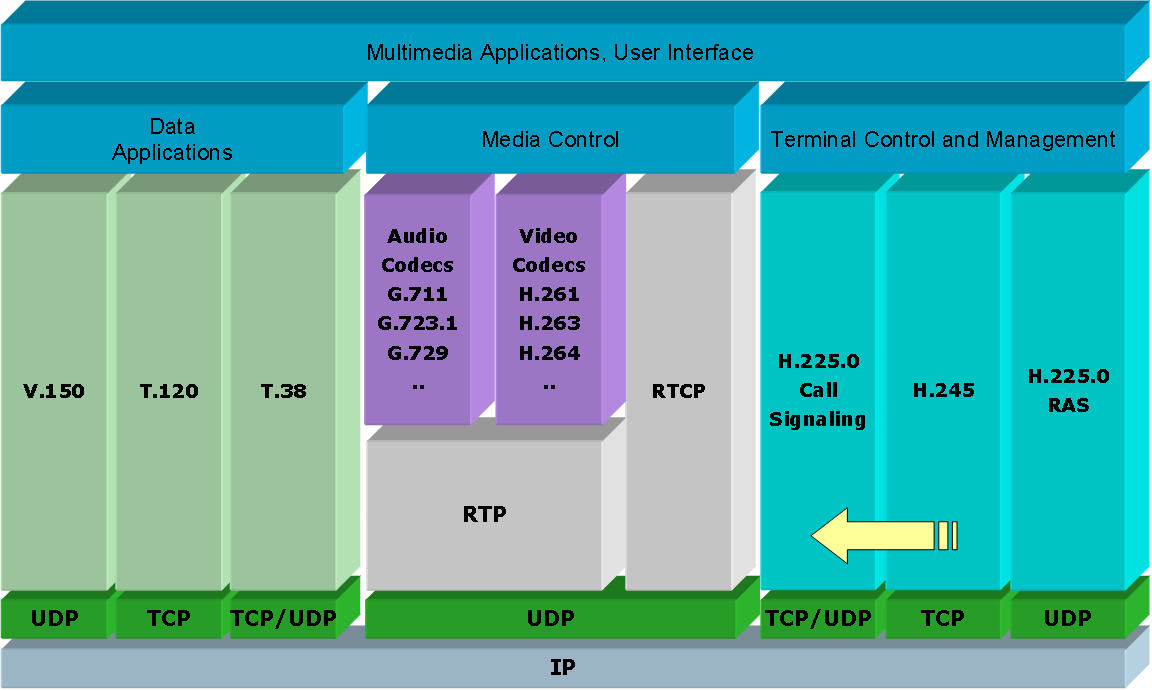
\includegraphics[width = \columnwidth]{figures/H323Stack.png}
    \caption{������ ���� ���������� H.323 ��~���� ��������� IP}
    \label{fig:H232stack}
\end{figure}

H.323 ��������� �������� ������ ��~4 ������������:\listnopagebreak
\begin{enumerate}
    \item������������~"--- ������������ ���������� �~���������� ��� ��������;
		\item���������� ��������� �����������~"--- �������� ������ �����������~������������ ���������� ��������� ������� (RTP);
		\item���������� �������� ������~"--- �������� �~������ ��������������� ����������, ����� ���~T.120 �~T.38;
		\item���������������� ����������~"--- �������������� ��������� ��~����������, ���������, ������� �������.
\end{enumerate}

����������, ����������� ���������� H.323, ����������� ��~��������� ����:\listnopagebreak
\begin{itemize}
    \item\keyworde{���������}{terminals};
		\item\keyworde{�����}{gateways};
		\item\keyworde{�����������}{gatekeepers};
		\item\keyworde{������� �������������� �����������}{multipoint control unit, MCU}.
\end{itemize}

\paragraph{��������.} ��������~"--- ��������� ���~����� ������ ���������� ����������, ��������� ��������� �������������� ���������� �~���������� �������� �����, �, ����~����������, ���������� ������������ �������� ������ ���~�����.

�������� ������ ������������ ���������:\listnopagebreak
\begin{itemize}
    \item\ H.245~"--- c����������� ���������� ����������;
    \item\ Q.931~"--- ������������ �~�������� ����������;
    \item\ RAS~"--- �������������� �~������������;
    \item\ RTP/RTCP~"--- ����������� �������� ���������� �����/�����;
    \item\ G.711~"--- ����� ���~�������� �������� ����������;
    \item\ ��������� ���������� H.450~"--- ���~��������� ������������ �~H.323 �������������� ����� ������������.
\end{itemize}

�������� ������� ���������~"--- ����������� ������������� ������� ���~�������������� ����� �~������ ����������, ������ ���~����������� ���������� ������������.

\paragraph{����.} ���� ��������� ���~������������ ���������� �~���������� ������� ���������.
����� �����~����������� ��������� ���������� �������������� ��~���� ���������� ���������� ��������� ����������, �������� ������ �~������� ����������.
����� ��~�������� ������������ ������������ ���� ��~��������� H.323, ��, ��� ��~�����, ���~������ ����������� ���~���������� ����� IP-��������� �~�������������� ��������� ���~����������� ����������� ������.

\paragraph{����������.} ����������, ���~���������� ���� H.323~"--- ���������� ���~���������, ����������� ��������� ������� ���������� ��������.
���~\keyword{�����} ��������������� ������������ ���� ��������� (����������, ������ �~MCU), ����������� ���~����������� �����������.
������~����� ���� ����� ���������� ��������� ����������������� ������������, �, ���~���������, ��������� ���.

�������� ������� �����������:\listnopagebreak
\begin{itemize}
    \item���������� ������� ��� �~��������� ������� �~������ ��������� IP;
		\item���������� ��������, ����������� ������� �~���� ��~��������� RAS;
		\item���������� ������� �����������;
		\item������������� ���������� ��������� �����~����������� ������~����.
\end{itemize}

������� ����������� �~���� ��~�������� ������������, ����~���������� ������� ����� IP-����� ��������� ����������� �������� \citebook{solomonovich2006ip}, ��~�������� ����� ����������� ������������ ����������� ������������.

\paragraph{MCU.} ������ ������������� �����������~"--- ����������, �������������� ���������-����� ���� ���~����� ����������.
������������ H.323 ������������� ��� ���� �����������:
\begin{enumerate}
    \item\keyword{���������������� �����������}, �~������� ����� ����� ������� �������� �����~MCU ��~����� <<�����-�����>>.
    \item\keyword{������������������ �����������}, ������������ ��������� ���������; MCU ����~������� ����������� �~����������� ����������.
    \item\keyword{��������� �����������}~"--- ������������ ��� ������� ������������.
\end{enumerate}

\subsection{���������� �.323}

��� ���������� ���� H.323 ����� ���� ��������� ���~� ����������� ����, ���~� �~���������-�����������~"--- ���������� ���������������� ������������.
���������-����������� ���������� ���������� ���~������� ����� IP-���������; ������������, ��������������� ���������� ��~��������� H.323, ���������� ��� ���������� ������ �������: Ericsson, Tedas, Lucent Technologies, Siemens, �isco, Avaya, Huawei, D-Link.

��~����������� �������, ������� ����� ������������� �~�� ���������� ������ �����������, ���~������ ����������� ��������� ���~��������� �����������, ���������� �������� ������� ��������� ���������� ��������� H.323~"--- H323Plus, ���������������� ��~�������� Mozilla Public~License \citeonline{h323plus}, ��~���� ������� �������� ������ ���������� �������: Ekiga, Asterisk, FreeSwitch.

\section{�������� SIP}

\subsection{������� �������� ���������}

\keyworde{�������� ������������� �������}{Session Initiation Protocol, SIP}~"--- ���������� �������� IP-���������, ������������� ������� Multiparty Multimedia Session Control (MMUSIC) ����������� ������ ��������� (\foreigne{Internet Engineering Task Force, IETF}).
�~������ ��������� ���� �������� ��������� ��������:\listnopagebreak
\begin{itemize}
    \item��������;
		\item������������� ��~������������� ������;
		\item������������ ����������� �������������;
		\item���������������� ����;
		\item������������� ���������;
		\item���������� �~���� ������������ ���������� ���������;
		\item�������������� �~������� ����������� ������������.
\end{itemize}

�������� ��~��, ���~� �������� ������������� ��������� ����� �������������� X.25, Frame Relay, IPX, AAL5/ATM \etc, ���������������� �������� ���� ���������� IP, TCP (���� 5060) �~UDP.

�������� SIP ����� ������-��������� �����������: ������ ����� �������, ������� �������������� ��~�������.
��������������� �~�������� �������� \keyworde{���������������� ��������� ������}{User Agent Client, UAC} �~\keyworde{���������������� ��������� ������}{UAS}.
���~������� �~UAC, �~UAS ����� ����� �������� �~\keyworde{���������������� ������}{User Agent, UA}, ������� ��~���� ������������ ����� ������������ ������������.
������������ ��������������� �������� ������~� ������������ �������������.

������� ��������� SIP ������� ��~�������� ��~��������� ����:
\begin{itemize}
    \item������-������;
		\item������ �������������;
		\item������ ����������� �������������� �������������;
		\item������ B2BUA.
\end{itemize}

\keyword{������-������} ������������ �������� ������������ �~����.
��~��~����� ����� �������� ��������� �~���������� ������������ ���������, ��������� ����~���� �������� ���������� �~����������� ���� <<Via>>.
���������� ��� ���� ��������: �~����������� ��������� �~���.
������ ��� ����� ������������ ������� ���������� �����: ������������� ��������� TCP ���~���������� ����������, ����������� ��������, ������������� �������� ���������� ����������; ��~�� �������� ��������, ���~������ ������� ����, ������� �������� ������~��� ������������.

\keyword{������ �������������} ������������ ���~����������� �������� �������������� ������������.
��~�������� ����� ����~����������� ������������, ����~������-�������, ��~�������� ��������� ������� ���������� ����� ������, ����� �������, ������ ������������� ��~�������� ���������� ����� ��.
���������� H.323, ��~����� ��~��������������, ����~������������ ��� ����� ������� ����� ����������� ��������, ���~����� ���~�� ������������ �����������, ������� �������� ����� ��~��������� SIP.

���~���� �������� ����, ����������� ������������ �������� ����� ��~�������� ��������� SIP, ������� ���������� ���������� ������� �������������� ������������ ���~�������� ��� ��������� �~���������� ��� ������� �������������.
���~����� ������� ����� ������������ �������� ��~\keyword{������� ����������� �������������� �������������}.
������������ ������ ���������������� ���� ������ ���~����������� �~���� �~������� ������� <<REGISTER>>.
����� ���� ������ �������� �~������-��������, ����� ������ ����� �������� \keyword{registrar}.

\keyworde{������ �����-�-�����}{back-to-back user agent}~"--- ������������� ������-�������, ���������� �~����� �~����� �����������, �������� ����� ���~����� ��~������ �������.
�~������ �������� B2BUA �������� �������������, ���~UAS ��~��������� �~���������� �~��� UAC ��~��������� �~������������ ����� ���������.
���������� ��������� ���������� �~������ ������ �~��� ������� ���������.
������ ��~���������� ���������� ��~������ ������������ ��������������� �~B2BUA, ���~� ��������� �����������, ����~� ���������������� ������ �������� �����������, ������� ����� �������������� ���~��������� �����:
\begin{itemize}
    \item�������;
		\item������� ������;
		\item�������������� ������������;
		\item���������� �����, �~�.\,�. �~������� ���������� ���������;
		\item�������� ��������� �����;
		\item�������� ������� ������ ������~������;
		\item\etc
\end{itemize}

�~�������������� ������ ��������� SIP ���� ����� 6~��������: INVITE, ACK, BYE, CANCEL, REGISTER �~OPTIONS, ���~��������������� �������� ��������, ����������� �~��������� ���������, ��~� ���������� �������� ���������� �~8~����� ����� ��������.
��� ��~�����, ����~� ����������� ������ ��������~�\'{�}����� �� ������������������ ������ ������������ ���~������������� ������������~��������� H.323 \citebook{meggelen2009asterisk}.
����� ����, ��������� ������� ��~������� ������������ ��~��������� HTTP, ��������, ��� 404 ���~�� ������������� ������ <<Not Found>>; ��� �������� ����������.

�������� SIP ���������� ��������� �������������.
����� SIP ������� ������ ����������� �����: ������ ����� �������������� ������������, ������ �����~"--- ����� ����, ����� ���~IP-�����, ����� ����������� ������ <<@>>.
���������� e-mail, �������������� ���������-��������, ���~��������� ���~������������� SIP-������� �~��������� ����������� �����, ���~� �~��������� ����, ��������� ���������� ����� ���~��� ����� ���~�������������.

\subsection{���������� SIP}

���������~�������� ���������, ���������� ����� ����� ��� ����������� ����������, ���~��������-��������, ���~� ��������, ������� ��~�� ����� ����������� �������� ����������.
���������-������� SIP �������� ����������� ���~������ ���������, ������� ��������� �~��������� ��~������ web-����������.
������ ����� ����������� ����������� ���~SIP ����� ���~�� �~������� ��������� H.323, ���~����������� ��������� ����������� ���������� ���~��������� ������������.

\section{��������� ���������� SIP �~H.323}

��� ���������, ����~� ������ ���������� ������, ���������� ������ ������ �~��������.
�������� H.323, ����� ������, ��� ������ ������������� �~������� ������������ ���������, �~�������� ����� �~����.
����� ������� �������� SIP ���������� ��� �~�������� ��~��������������� ���������, ������� ����������� ��������� ��� ������������ �������� ������.
������� �������� SIP �������� ���������������� ���~����������, ����������� �~����������� ���������� ����� �����.

���������~��������� ����������� �����������, �������� ������������� ���������� ����������� �����, �� ��~������ ������ ������������� �������� �~������� ���.
�������� ������� �������, ��� ��~�����, ����������� �~����������� �����������, ���~��� �������� H.323 ���������� ����� ������� ������� �~������������ �������������� ����������� ����������� MCU.
�~������ �������, ������������������ ��������� H.323 ������������� ������ ������������ �������� ���~�������������.
����������� ����������� �������� ��������� H.323 ���������� �~� ������ ��������, ���, ��������, �������������� �~����� �������������, �������� ���~���������.
����� ����������� ��������� SIP ����������.

�������� ������� �������� �����~����������� ����������� �~������ �������������� �����.
����� ����� �������� ������������ ��������� SIP, ��������������� ����������� ����������� ����� ������� ��������, ���~����� �������������� ����������� �~����������� call-center; ����������� ������� ����������� �~������������ �������; ���������� ��������� ����������� �������������.

������ ������������ ������������� ��������� SIP �������� ��� �������������, ������� ��~������ ���� ��������� ��������.
���������������� ������� ������ ������������ ���������, ������������� ����� ������ ������ ��������� SIP, ���~������������ ������� �~�������� ������������� �~������.
����������� ��������� ��������� H.323 ����� ������, �~������� ������������� ����� �������������� ���������� ������~����� ������� ���������, ���~����� ��������� �~��������������� ������������, ���������������� ������� ���������������.
���������� ����� ���������������� �~�������� H.323 ����� �������� �~������������� ��������� ���� ����������, �, ���~���������, �� ����������; �������� SIP~�� �������� ��������� ����������, ������ ����� ���� �������� ���������� ���� ��~�����.
SIP ��~������������� ������, ������� �~��� ��~�������� ������� ������������� ���������� �~�������������� ����������� �����������.

���������������� ����� ��~���� ��������� H.323 ����������� ������ ������������ ��������� ����������~"--- ���~������ ����� ���� ���������� ��������� ������ �����������, ���������� ����������� �������� ������ ���������� ����������� ������� SIP, �������� ��~����� ��������� �������.
�~������ �������, ��-��~���������� ���������� �������� �~�������� �������� SIP ����� ������������ �~���������� �~����.

����� ������������ ���������� �������� ������������ ��������, ������������ ����������������� ������ IP-��������� ���~��������.
������������ �������� ��������� SIP ��������� ����������� ��������� ����� ������������ ���������� ��~��������� �~���������� H.323: SIP ���������� ���� ������, �~�� ����� ���~H.323 ���������� ������������ ����� �����������, ������� ����~� ����� ��������� ���~������ ��������� ������, �� ����� �������~�\'{�}�����.

���~��� ���� �������� ����, �������� SIP ���������� HTTP-�������� ��������� ������ ���������, ���������~���� ������ ��� ������ ����� ���~������������, ���~��� ��~���������� ������������ ����������, ���~�������� �~��������� H.323, ������������ ���� ASN.1.
�~������ �������, ��������� ��������� �~�������� ���� �������������� �������, ��~� ����������� �������������� ��������� ��� ������������ ��������.

�~����� ������ ������������ ������������� ����� ���������� ���������; ����������, ���~��� ���� ��������, ��������� ��������� ��������-��������, ��������������� ���������� ����������� ��������� ���~���������� SIP �~H.323.
����� �������, ������� �������� ������� ����������� ��~��������� ����, ��������������� ������.
������ ��~�������������� �������, ���~��������, ��������� ��~����� IP-��������� ��~������� ��������-�����, �������� �������� SIP, ���������~�� ������������� ������� ������ �����, �~������� ��~���������� ������ ����������� ����������.
��������, ����� ��������������� ������ ������� ��������� �~�������� ������, ���� �������� �������� H.323, ���~��� ��~����� ��������� �~������������ ����������, �~������� ������ ��������� ������������ �~����� ������������, �~�����.

\section{������ �������}

��������� H.323 �~SIP, �������� ��~���� ������������������, ��~�������� ������������� ��������� ���~IP-���������.

\subsection{�������� MGCP}

\keyworde{�������� ���������� ������������ �������}{Media Gateway Control Protocol, MGCP}~"--- ��������, �~������ �������� ����� ���� ������������ ����� ��:
\begin{enumerate}
    \item������������ ����, ����������� ������� �������������� ������� ���������� ���� �~��������� ���~�������� ��~����� IP ��� �~�������;
		\item��������� ���������� ������;
		\item���� ������������, �������������� ����� ���������� ����������� �����~���� �~����������� ���������� ������.
\end{enumerate}

��~���� ����� ������������ ����������� ������������ ���������� �������� ��~���������� ������, �, ���~���������, ����������� ���� �~����������� �������� ���������������.
�\'{�}����� ������������ �~���������� �~���� ������ ���� �������� ������������ �~H.323, �~���������, ������ MGCP ������� ���������� ������� �������������� Nortel Networks;
����~������� ������������ ������� ������� ������������� H.323 �~������������ ����� IP-���������.

����������� ��������� MGCP �������� ��� ���������������, ����������~������� ������������ ��������� �������������� ���������� �������������.
��~���������� �������� �~������ �~������������� ������������, ���������� \emph{de facto} �������� ������������� ���������� ������� ���~����������� SIP.

\subsection{Skype}

\keyword{Skype}~"--- ���������� ����������� �������� IP-���������.
������ ���� ��������� �������� ��~��������� \keyworde{�����-�����}{point to point, P2P}, \ie~������ ��~������� ���������������� ��������.
�������� ������ �����~����� �������������� ���������������� �����~���������� ������ �������������, ���~��������� ����������� ���� �~������ ������������� ��������� ���� ���~�������� ������ ������.
������������ ���������������� ����� �������� ������ �������������, ��~������� �������� ������� ������ ������������� ����.

���������� �������������� ���������� Skype �������� ����������� (������ ���� ����������� ���~��� ����������� ���������), ������� �������� ���������� ��~���� ����� ����������� �������������.
��� ��~�����, ��� ���������� �������� �~����� ������������ �����������.
�������� ��� ��������� ������, ���~������������� �������� ������� �~������������������ ����������; �����~���������� ���������� ������ Skype ��������� ����� ��������� ���� �����������.
���������� ������ ��������� ���� P2P ������� ���������� �������� ���������� ������������ �������������, �~������ ��������� ���� ������������ ����������� ��� ����� �������� ����������� �~�������� ����� ����� �����������.
��~�������� ��~��� ����������, Skype ��������� ���~� �������������� �������������, ���~� �~�������������, ��������~� �������� �~������� ������������ �����������.

%% Анализ рынка
\chapter{Анализ рынка}

Рынок IP-телефонии~"--- развивающийся рынок IT-услуг.
В~2012 году объём всего рынка в~России составил 4,59 млрд рублей, в~2013 ожидался рост до~5,35 млрд рублей.
17\% населения России (27 млн человек) постоянно используют технологии IP-телефонии, и~с течением времени эта цифра постепенно увеличивается.
Скорость увеличения, однако, ограничена отсутствием необходимости в~сервисах IP-телефонии у~многих абонентов.
Стоит отметить, что~многими экспертами рынок IP-телефонии в~России оценивается как~низкий \citeonline{discovery}.

\section{Частный сегмент}

Услуги IP-телефонии частного сегмента можно разделить на~несколько типов:
\begin{itemize}
    \itemуслуги операторского класса, поставляемые в~пакете с~услугами широкополосного доступа, телевидения \etc;
		\itemуслуги Over-the-Top, поставляемые сторонними компаниями.
\end{itemize}

Как~правило, услуги первого типа предоставляются <<классическими операторами>> связи, такими как~Билайн, Стрим, Акадо и~другие.
В~последнее время, однако, многие пользователи Интернета выбирают IP-телефонию второго типа, а~именно технологии Skype (Microsoft), FaceTime (Apple), GoogleTalk (Google) \etc.
Преимуществом этих технологий для~пользователей является повышенная мобильность, распространённость технологий по~миру~"--- можно звонить в~любую точку мира по~одинаковой цене.
Как~правило, эти технологии несовместимы между~собой, и~поэтому пользователю приходится в~той или~иной мере пользоваться ими всеми.

Технологии сторонних компаний завоёвывают всё большую популярность относительно~услуг ТфОП: так~из-за~этого фактора, например, по~итогам 2012 года ожидаемое снижение доходов европейских сотовых операторов составило от~1,5\% до~4\%.
Наиболее заметное снижение выручки заметно в~секторе дальней связи, где в~России операторы фиксированной связи за~2012 год потеряли около~25\% выручки.
В~связи с~этим, операторы всё больше и~больше уделяют внимание собственным услугам IP-телефонии, а~также снижению цен на~услуги <<классической>> телефонии.

\section{Корпоративный сегмент}

Основная доля российского рынка (73\%) IP-телефонии приходится на~корпоративный сектор, из~которой 45\% составляют услуги виртуальных АТС.
В~этом сегменте, согласно прогнозам J'son \& Partners Consulting, объём рынка к~2016 году увеличится до~3,8 млрд руб, а~среднегодовой темп роста рынка за~период с~2010 по~2016 год составит 30\%.
Соответственно, ожидается снижение доходов операторов фиксированной телефонии как~устаревающей технологии; средняя выручка на~одного пользователя с~использованием новой технологии сравняется с~этим показателем для~фиксированной телефонии в~2015 году \citeonline{jsonmarkets}.

Согласно результатам проведённого исследования \citeonline{jsonmarkets} наибольший спрос на~виртуальные АТС зафиксирован у~компаний малого и~среднего бизнеса, занимающихся ритейлом/продажами, телекоммуникациями, IT и~промышленных компаний; эти компании составляют 45\% рынка услуг виртуальных АТС.
22,5\% рынка составляют следующие сектора крупного бизнеса: телекоммуникации, IT и~промышленные компании, а~так~же государственные компании и~учреждения.

%% Заключение
\addchap{����������}

IP-���������~"--- ����������, �������� �~����� ���~������� �������������, ���~� ������������� ���������~��������� �������� ��������:
\begin{itemize}
    \item�������� ������ ���������� �~������ �������� ������;
		\item��������������� ����������� ���������� ����� ������ �����������;
		\item������ ��������� ����� ���~��������� ������������.
\end{itemize}

������� ����������� ���������� �~��������� IP-��������� ��������� �������� ��������� ������� � ����������, �~�������������, �~�������� �����.
���, ��������, ����� ������� ������ IP-��������� ������������� ����������� ���������� �~������������� ����������� ������; ������ �������, ��������, ��������� ������� ������� <<�~����>>.

����� IP-��������� �� ��� �����������, ������� ���������� ������������ ���~��������� ������������ �������, �� ��������� �~�������� ����� ������� �������� ���������� �������.


%% Список литературы
\addchap{Список источников и~литературы}

\bibliography{../../global}

\setbiblabelwidth{99}
\bibliographystylebook{../../configs/gost2008s}
\bibliographybook{../../global}

\setbiblabelwidth{99}
\bibliographystyleonline{../../configs/gost2008s}
\bibliographyonline{../../global}


%% Приложения
\appendix
% Делаем нумерацию приложений русскими буквами
\renewcommand{\thechapter}{\Asbuk{chapter}}

\end{document}
